\documentclass[12pt, oneside]{article}   	% use "amsart" instead of "article" for
\usepackage[left=2.7cm,right=2.7cm,top=2.7cm,bottom=2.7cm]{geometry}	

\usepackage{graphicx}		
\usepackage{amssymb}
\usepackage{amsmath}
\usepackage[font=normalsize]{caption}
\usepackage{subcaption}
\usepackage{float}
\newcommand{\reffig}[1]{Figure \ref{#1}\hspace{2pt}}



\title{Factors Affecting Agriculture in Sahara }
\author{Kun Zhou 204688165}
%\date{March 12, 2016}						% Activate to display a given date or no date

\begin{document}
\maketitle

\begin{abstract}
Agriculture is always the key development in the rise of human civilization.  To improve agriculture efficiency is an emergency, especially in Africa.  Thus, researching geospatial factors for Africa South of the Sahara helps utilize resource in different areas to improve agriculture.   I analyzed 66322 observations with 96 variables from a multidisciplinary geospatial database.  I mainly applied principle component analysis, different regressions and correspondence analysis to study relation within observations.  Based on statistical analysis, the variance of livestock density is proportional to itself.  Total least square can predict livestock density given natural factors. The ports, which contribute less to agriculture, are classified.  Last I talked about some problems that need to be overcome for further study.\\
\end{abstract}

\section{Introduction}
Agriculture has an unreplaceable position from the evolution of human from ancient times to 21st century.  Thanks to industrial revolution, human believed starvation was overcome one time.  However, with the rapid growth of population, this problem become more severe than before.  By the end of 21st century, the total population in the world is estimated to be 11.2 billion, according to UN (2015)\cite{World Population Prospects}.  Improving agriculture is an emergency.  \par
\vspace{4mm}
My goal was first to study which factors influence (referred as a $n*p$ matrix $X$) the livestock density, farm system and production vale per hectare (referred as a $n*m$ matrix $Y$). These are important elements for evaluating agriculture.  Then I tried to found the quantitative relation between $X$ and $Y$ with statistical method such as regressions, analysis of variance and correspondence analysis. Besides, I also tried to extract main information from $X$ with principle component analysis so that a smaller size of new factors can be used in further study.  Random forest is introduced shortly.\par
\vspace{4mm}
The data is collected from a multidisciplinary geospatial database for Africa South of the Sahara (HarvestChoice\cite{HarvestChoice}).  After deleting missing data, it contains 66322 observations with 96 variables.  I classified the data into 4 parts which are then divided into subparts.  The 4 parts are natural factors, social factors, agriculture and location.  Each part contain multiple factors as follows:\\
\textbf{Natural factors}
\begin{itemize}
  \item Ecology: ecological zones (class)
  \item Climate: mean of growing period (days), coefficient of variation of growing period (percent), mean of Annual rainfall (mm), coefficient of variation of annual rainfall (percent)
  \item Land cover and use: cropland (ha)
  \item Soil resource: 12 different kinds of makeup of soil (percentage), content of organic makeup at 6 different depth (per mile)
\end{itemize}
\textbf{Social factor}
\begin{itemize}
  \item Market: areas that share the nearest market (class)
  \item Port: areas that share the nearest port (class)
  \item Travel: mean travel time to human settlement of 20,000 or greater population (hour)
\end{itemize}
\textbf{Agricultural evaluation}
\begin{itemize}
  \item Farming System: farming systems name (class)
  \item Livestock: density of cattle, poultry, goat, pig, sheep(head/sq. km)
  \item Production: 47 different kinds of economic botany (mt)
  \item Value of production: food, non-food, total value production per hectare (Int\$/ha), food non-food, total value production (Int\$)
\end{itemize}
%\textbf{Life quality}
%\begin{itemize}
%  \item Health and nutrition: Body Mass Index (index), rural child mortality with different ages (per thousand), underweight (percent)
%  \item Income and poverty: rural Gini (index), poverty (USD per capita per expenditure)
%\end{itemize}
\textbf{Location}
\begin{itemize}
  \item Location: longitude (degree), latitude (degree)
\end{itemize}
%This partition is based on the following consideration.  Natural factors directly influence agriculture but less influence modern human living. (Because air condition, cars and so on compensate disadvantages brought by nature factors.)  Social factors also directly influence agriculture since farms nearby cities are invested more to maintain cities themselves while farms far away are less concerned.   And social factors do contribute significantly to life quality, but the research is on how agriculture influences life quality.  Therefore, I didn't consider them when analyzing life quality.  Based on above, I focused on how agricultural evaluation is affected by nature and social factors and how it affected life quality.\par
For this report, I mainly researched relation within soil resource, relation within natural factors, livestock density and farm system and relation between social factors and production value.  The next two sections is to discuss my findings.  Then a followed section is to discuss the problems and further improvements. 

\section{Natural Factors}
 For this section, I refer natural factors as $Z$, farm system as $F$ and livestock density as $Y$.  To clarify, (cattle, poultry, goat, pig, sheep) = $(y_1, y_2, y_3, y_4, y_5)$ where $y_i$ is column vector.
 
\subsection{Factors of Soil Source}
There are 19 factors about soil resource.  It is reasonable that some microelements have overlapping effects and the amount of organic makeup at deep correlated with it at surface.  So apply principle component analysis on soil resource.  The square roots of eigenvalues are shown as follows:
\begin{verbatim}
> soil_resource.pca$sdev
 [1] 64.1681233 46.9182038 38.7931878 22.7260678 19.5677735 18.5294155
 [7] 14.8032608 13.1016995 12.1036033  8.2265235  5.2376957  4.1924612
[13]  2.9366441  2.7549136  1.4100579  1.1324821  0.8797779  0.4805803
[19]  0.2840738
\end{verbatim}
Actually the sum of first 5 eigenvalues make up 89.58\% of the total sum.  In other worlds, 5 new factors can be used to illustrate 89.58\% information of the 19 old factors.  If all variables of soil source are used in regression, multicollinearity could arise.  So one cannot tell which facotrs will contribute to agriculture and which not.  For exmaple, if a 1-unit total effect of sodium and potassium increased production by 1 ton, the result could be that sodium and potassium increased production by 0.1 and 0.9 repsectively or by -0.1 and 0.11 respectivley.  Thus, although using new factors can lose some information, new factors avoid multicollinearity.\par

\subsection{OLS for Natural Factors and Livestock Density}
I performed ordinary least squares regression (OLS) to predict livestock with natural factors after applying PCA.  The variance of $Y$ is assumed to be constant. The formula $\beta = (XX^\top)^{-1}X^\top Y$ is true even when Y is a matrix.  What's more, performing OLS on $Y$ and performing OLS on $y_i$ separately have the same effect.
\begin{equation*}
\begin{split}
(\beta_1, \ldots, \beta_m)& = \beta_{n*m} = (XX^\top)^{-1}X^\top Y = (XX^\top)^{-1}X^\top (y_1, \ldots, y_m)  \\
&=((XX^\top)^{-1}X^\top y_1, \ldots,(XX^\top)^{-1}X^\top y_m)
\end{split}
\end{equation*}
Here is the result of sheep density ($y_5$). Other results are similar.
\begin{verbatim}
Response AD05_SHEE :

Call:
lm(formula = AD05_SHEE ~ LGP_AVG + LGP_CV + pre_cv + pre_mean +
    ELEVATION + AREA_CR_LC + PC1 + PC2 + PC3 + PC4 + PC5,
    data = cbind(agriculture.c.tra, climate_geology.p.tra))

Residuals:
    Min      1Q  Median      3Q     Max
 -53.71   -9.64   -4.67    2.97 1281.24

Coefficients:
              Estimate Std. Error t value Pr(>|t|)
(Intercept)  1.100e+01  1.121e+00   9.808  < 2e-16 ***
LGP_AVG     -5.081e-02  3.643e-03 -13.948  < 2e-16 ***
LGP_CV      -8.129e-03  3.603e-02  -0.226 0.821500
pre_cv      -2.124e-03  4.025e-02  -0.053 0.957921
pre_mean     3.935e-03  7.277e-04   5.408  6.4e-08 ***
ELEVATION    1.310e-04  2.901e-04   0.452 0.651613
AREA_CR_LC   5.048e-03  6.437e-05  78.420  < 2e-16 ***
PC1         -3.223e-02  2.300e-03 -14.009  < 2e-16 ***
PC2          3.326e-02  3.136e-03  10.603  < 2e-16 ***
PC3          2.526e-02  3.195e-03   7.906  2.7e-15 ***
PC4          6.821e-03  5.637e-03   1.210 0.226225
PC5          2.357e-02  6.452e-03   3.654 0.000259 ***
---

Residual standard error: 29.23 on 59689 degrees of freedom
Multiple R-squared:  0.1481,	Adjusted R-squared:  0.148
F-statistic: 943.7 on 11 and 59689 DF,  p-value: < 2.2e-16

\end{verbatim}
we get some significant parameters.  Plant growing period is negatively correlated with sheep density.  This result matches our intuition. If grass is plenty and renewable with short growing period, sheep won't starve.  The rainfall is positively correlated with sheep density from the result, because sheep cannot die for thirsty with plenty water. Also I learned coefficients of variation of growing period and rainfall and elevation don't affect density significantly.  But for the cattle density, all parameters except PC5 (which is the fifth combination variable of soil source) are significant.  And pigs density is not influenced by growing period (p-value is 0.3070)  Considering the 5 different density, I concluded that growing period is negatively correlated with $Y$, cropland is positively correlated with $Y$.  Other factors don't have consistent effect on $Y$.   \par
\vspace{4mm}
Now, diagnose the linear model.  \reffig{ols_res} shows residuals are not random.  Instead they increase linearly with the increasing of $y_5$.  And in \reffig{ols_fit} the fitted values are not much correlated with sheep density and the correlation is 0.5185.  Besides, 14.39\% of fitted values are below 0 which is impossible in real life.  So I need to improve OLS with two assumption: 1) $Y$ is not normal distribution and its variance is linearly correlated with livestock density. 2) Fitted values are no less than 0 or at least only a few fitted values (under 5\%) are less than 0. \par
\vspace{4mm}
\begin{figure}[H]
        \centering
        \begin{subfigure}[b]{0.475\textwidth}
            \centering
            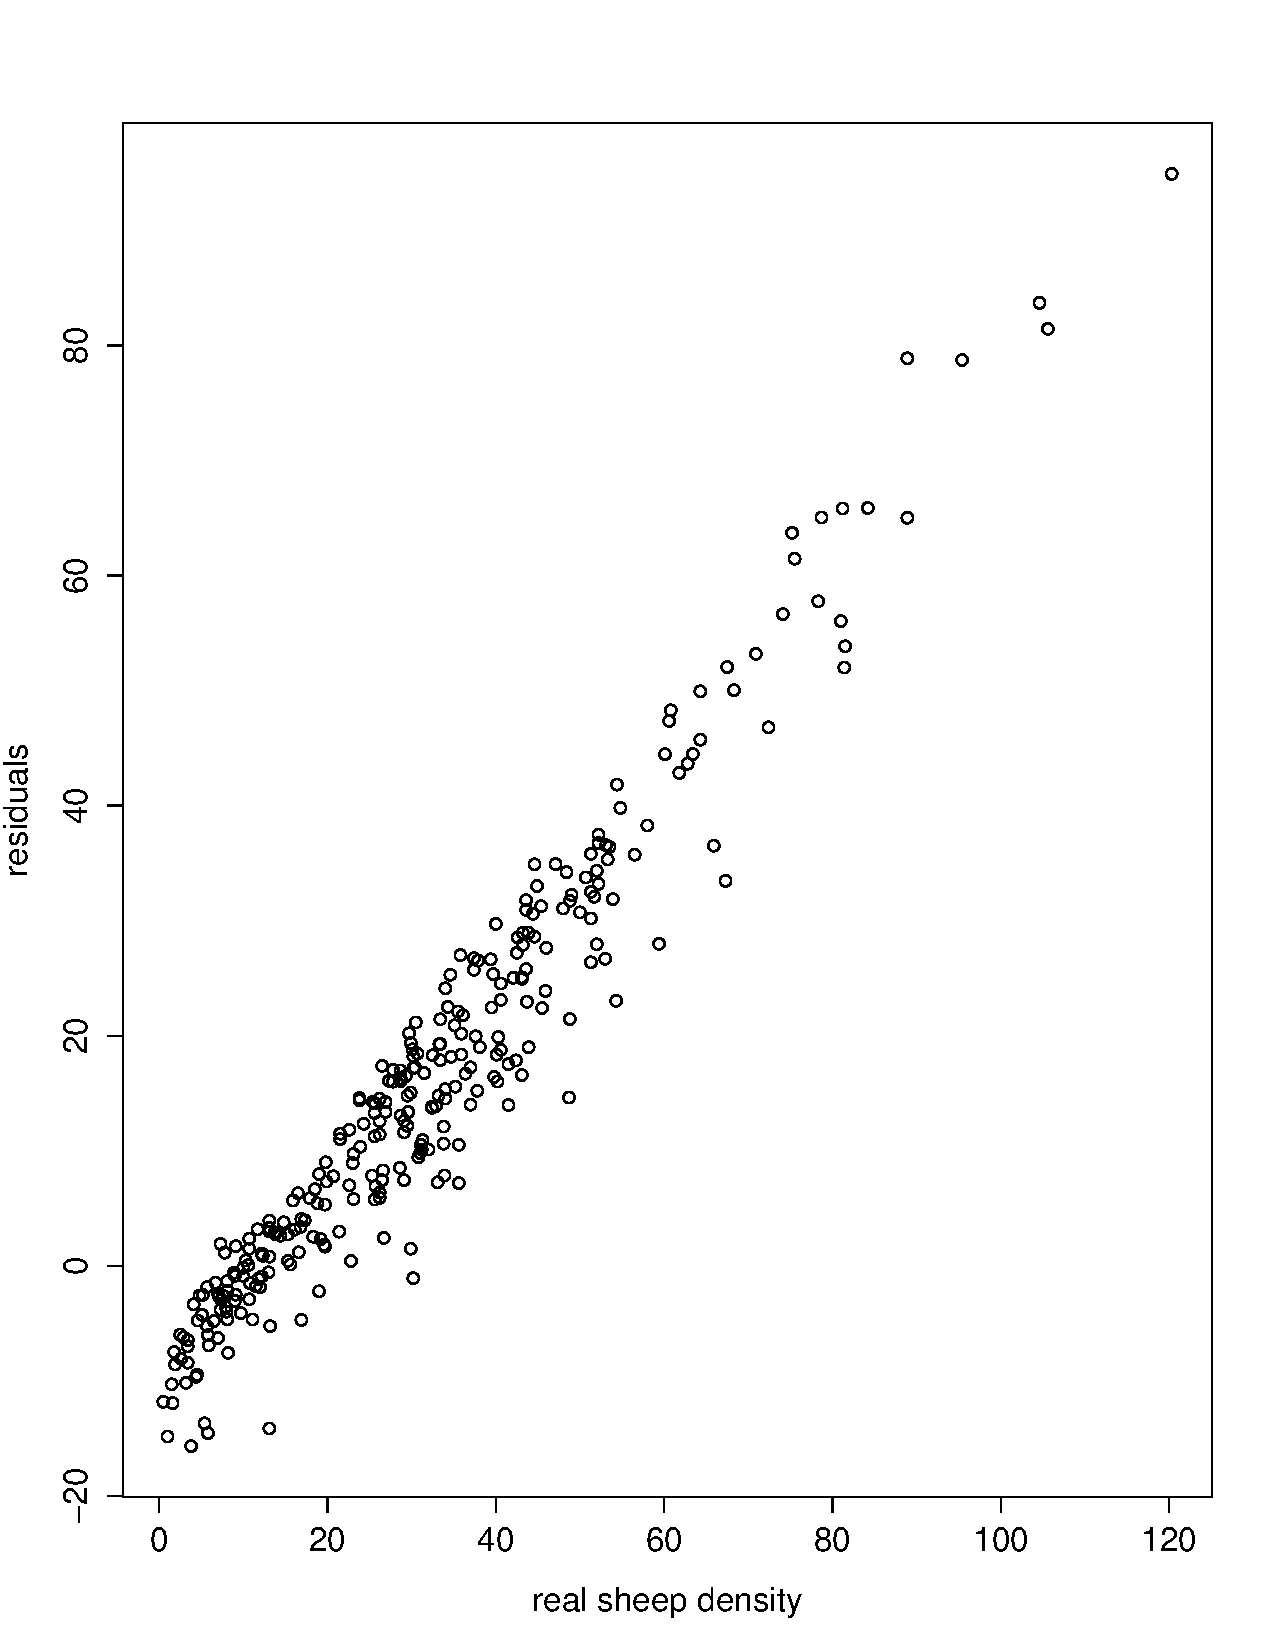
\includegraphics[width=\textwidth, height=6cm]{ols_res.pdf}
            \caption{residual plot with first 300 points}\label{ols_res}
        \end{subfigure}
        \quad
        \begin{subfigure}[b]{0.475\textwidth}
            \centering
            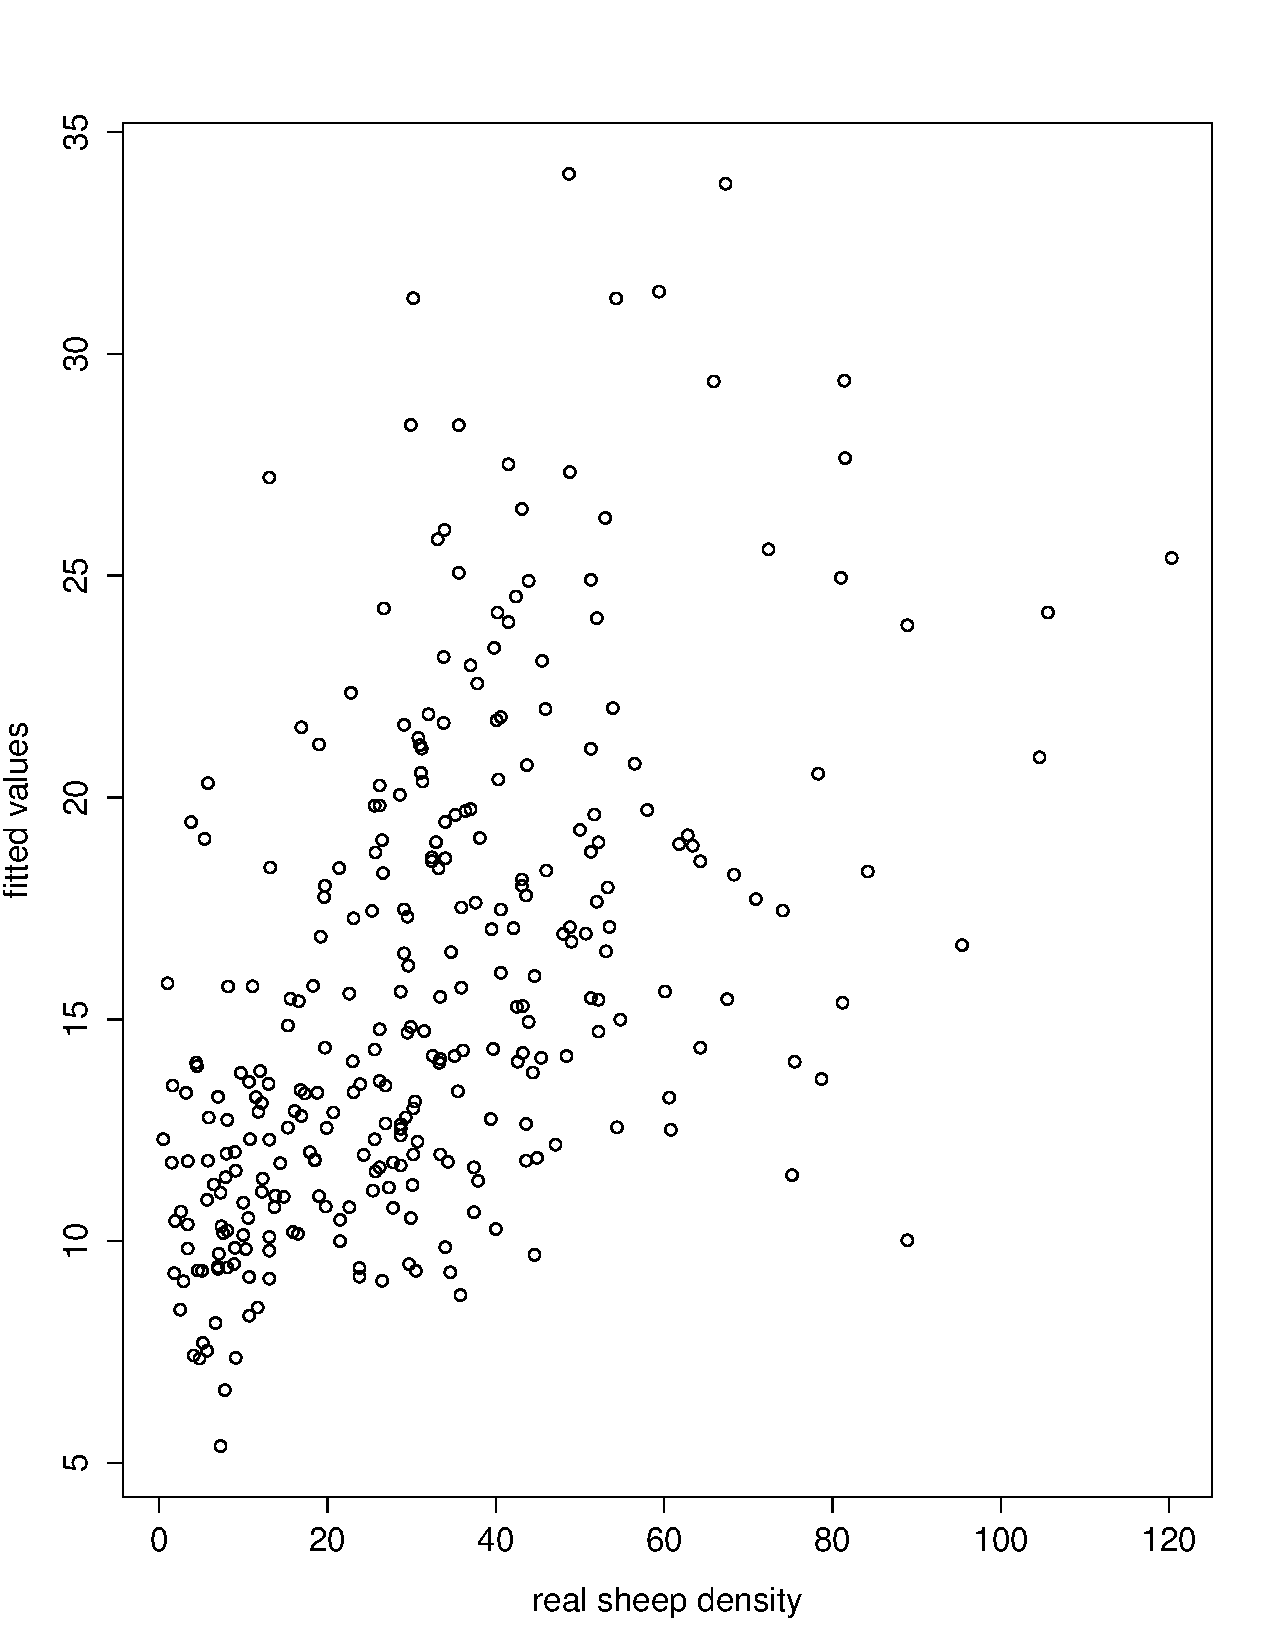
\includegraphics[width=\textwidth, height=6cm]{ols_fit.pdf}
            \caption{fitted value plot with first 300 points}\label{ols_fit}
        \end{subfigure}
        \caption{}
\end{figure}

\subsection{Attempt to improve by Logistic Regression}

For the second assumption, it can be proved mathematically that there is no continuous monotonically increasing function, which can mapping $[0, \infty]$ to $[-\infty, \infty]$.  So, we cannot think up a transformation to map $y_i$ to $[-\infty, \infty]$ so that fitted values after mapping can safely be negative.  Here I first used logistic regression (LR) to classify whether sheep density is zero.  If it is not zero, I applied log function to $Y$ and then OLS.  Here I briefly introduce LR.  Assume we have data $(A_i, B_i)$ where $B_i$ is either 0 or 1.  Assume $B_i $ follows binomial random variable with probability $p_i$. Then we establish model like:
\begin{align*}
E(B_i|A_i) = p_i = \frac{1}{1+e^{-A_i^\top \beta}}
\end{align*}
When predicting, if the predicted $\widehat{p}_i$ is greater than 0.5, $A_i$ is classified as 1 and otherwise 0.  The following is the logistic regression output of sheep density ($y_5$).
\begin{verbatim}
Call:
glm(formula = sheep.disc ~ ., data = data)

Deviance Residuals:
    Min       1Q   Median       3Q      Max
-1.3109  -0.4382   0.1673   0.3082   0.8964

Coefficients:
              Estimate Std. Error t value Pr(>|t|)
(Intercept)  1.102e+00  1.575e-02  69.963  < 2e-16 ***
LGP_AVG     -3.845e-04  5.118e-05  -7.513 5.87e-14 ***
LGP_CV       1.445e-02  5.062e-04  28.552  < 2e-16 ***
pre_cv      -1.725e-02  5.655e-04 -30.510  < 2e-16 ***
pre_mean    -2.045e-04  1.022e-05 -19.998  < 2e-16 ***
ELEVATION   -3.192e-05  4.076e-06  -7.832 4.86e-15 ***
AREA_CR_LC   5.200e-05  9.044e-07  57.496  < 2e-16 ***
PC1         -1.439e-04  3.232e-05  -4.452 8.54e-06 ***
PC2         -1.743e-03  4.407e-05 -39.556  < 2e-16 ***
PC3          3.440e-04  4.488e-05   7.664 1.82e-14 ***
PC4          2.051e-04  7.919e-05   2.589  0.00961 **
PC5          1.654e-03  9.064e-05  18.245  < 2e-16 ***
---
(Dispersion parameter for gaussian family taken to be 0.1686968)

    Null deviance: 11890  on 59700  degrees of freedom
Residual deviance: 10069  on 59689  degrees of freedom
AIC: 63191

Number of Fisher Scoring iterations: 2
\end{verbatim}
Then extract observations where elements of $y_5$ is larger than 0 and apply log function. so I get $\log(\widetilde{y}_5)$ and apply OLS to it.  Meanwhile, I wished log function could make variance constant, which is true after try.
\begin{verbatim}
Call:
lm(formula = log(AD05_SHEE) ~ LGP_AVG + LGP_CV + pre_cv + pre_mean +
    ELEVATION + AREA_CR_LC + PC1 + PC2 + PC3 + PC4 + PC5, data = data)

Residuals:
    Min      1Q  Median      3Q     Max
-5.8768 -1.0925  0.1098  1.1454  6.3841

Coefficients:
              Estimate Std. Error t value Pr(>|t|)
(Intercept)  1.568e+00  7.034e-02  22.290  < 2e-16 ***
LGP_AVG     -3.087e-03  2.551e-04 -12.103  < 2e-16 ***
LGP_CV       2.821e-02  2.298e-03  12.276  < 2e-16 ***
pre_cv      -2.008e-02  2.654e-03  -7.566 3.94e-14 ***
pre_mean    -2.255e-04  4.679e-05  -4.819 1.45e-06 ***
ELEVATION   -1.030e-04  1.911e-05  -5.393 6.98e-08 ***
AREA_CR_LC   3.059e-04  3.905e-06  78.349  < 2e-16 ***
PC1         -8.355e-03  1.497e-04 -55.799  < 2e-16 ***
PC2          2.274e-03  2.127e-04  10.694  < 2e-16 ***
PC3          2.144e-03  2.138e-04  10.028  < 2e-16 ***
PC4          1.299e-03  3.847e-04   3.378 0.000732 ***
PC5          9.244e-03  4.289e-04  21.551  < 2e-16 ***
---

Residual standard error: 1.649 on 43300 degrees of freedom
Multiple R-squared:  0.3333,	Adjusted R-squared:  0.3331
F-statistic:  1968 on 11 and 43300 DF,  p-value: < 2.2e-16
\end{verbatim}

All parameters are significant in OLS and LR.  Only the sign of "PC2" in OLS and in LR is not consistent.  This parameter is the combination of soil source.  Whether it is reasonable needs scientific check.  Other parameters are consistent.  For instance, Longer growing period makes LR prone to classify density as zero.  If not, it makes OLS to get a smaller density with negative parameter.  Finally, I noticed that the parameter of rainfall in OLS is changed to negative sign in this model.  It is against my intuition.  Maybe humid environment is not good for livestock.  It should be checked in scientific survey. \par
\vspace{4mm}

Still the model should be diagnosed. For LR, I use test set (which has different elements when I performed LR and OLS) to calculate the accuracy, 73.88\%.  The classification accuracy is somehow low.  So I tired to add interaction among formula, but it doesn't improve accuracy  (0.7676)much. On the other hand, although with data $y_5>0$, \reffig{glm_ols_fit} demonstrates the predicted values are improved, \reffig{glm_ols_res} shows residuals still have linear relation with $y_5$.
\begin{figure}[H]
        \centering
        \begin{subfigure}[b]{0.475\textwidth}
            \centering
            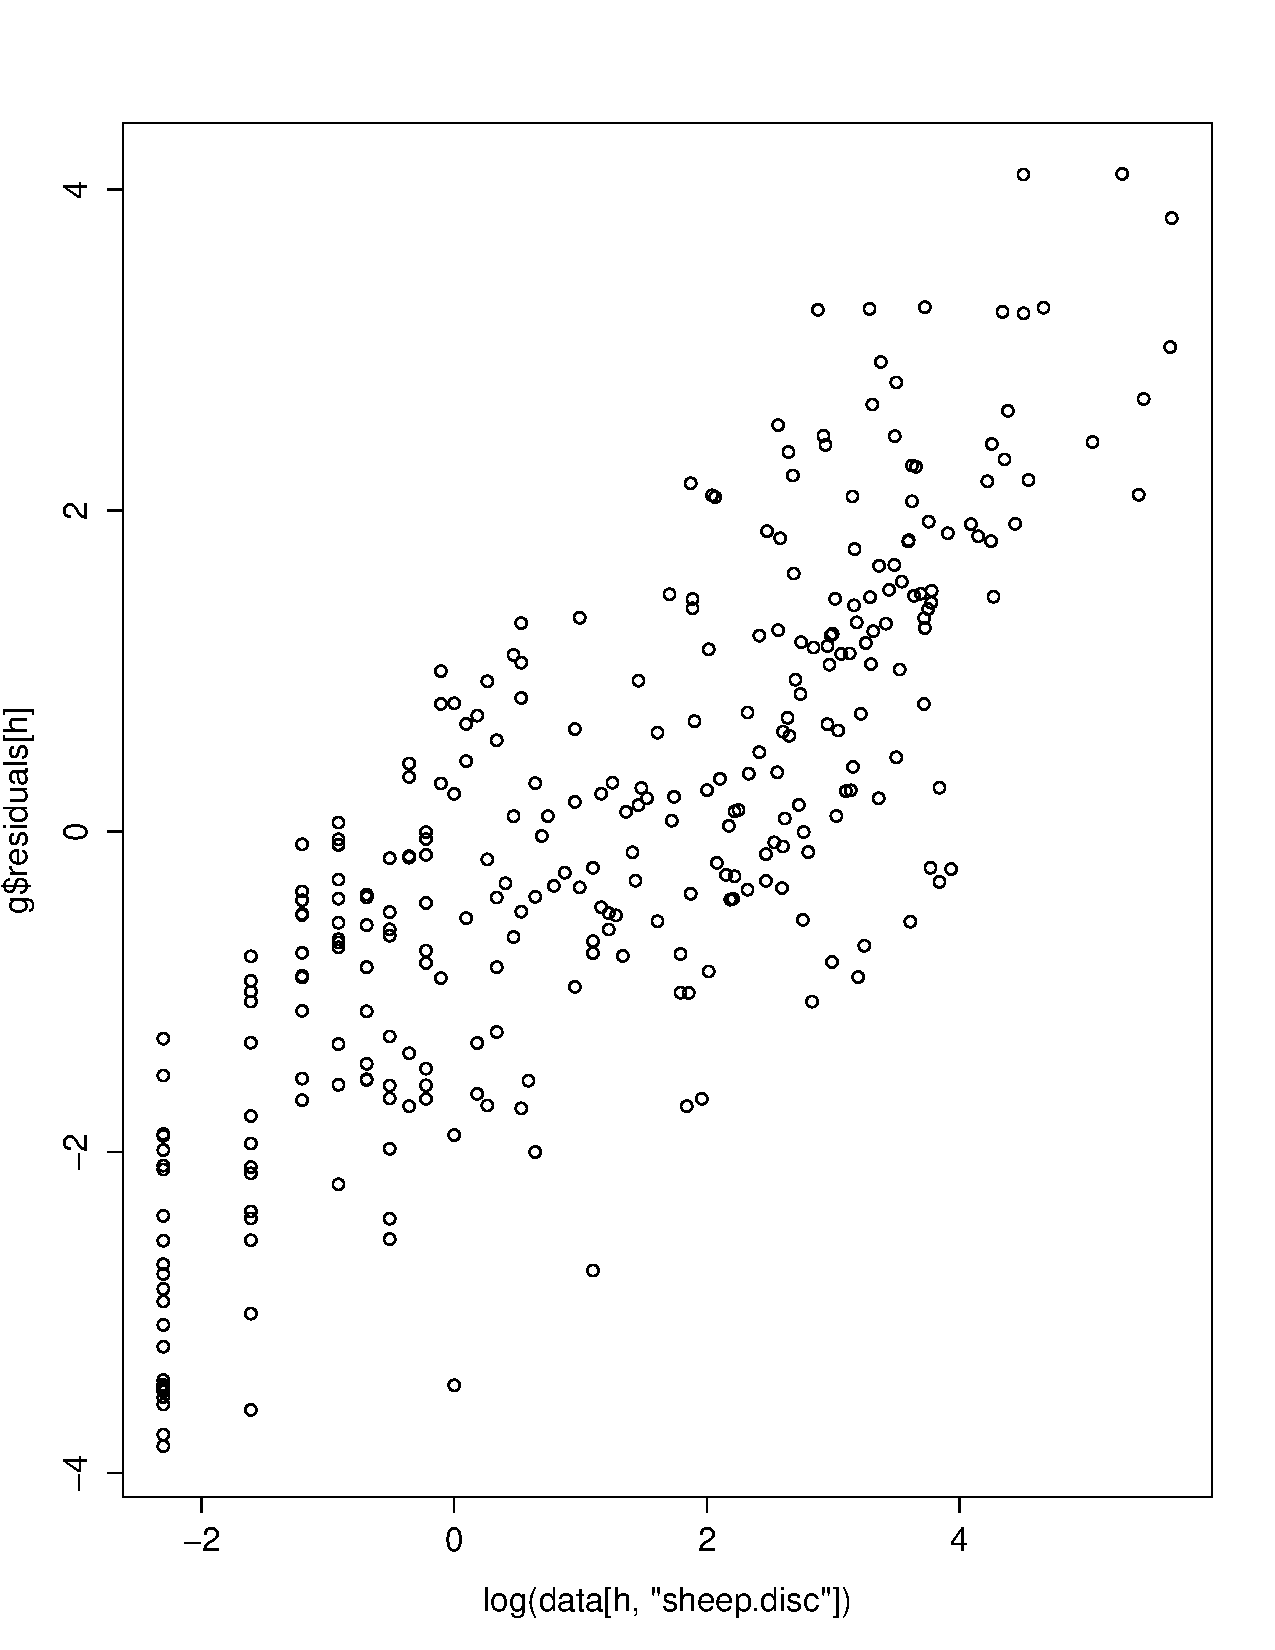
\includegraphics[width=\textwidth, height=6cm]{glm_ols_res.pdf}
            \caption{residual plot with first 300 points}\label{glm_ols_res}
        \end{subfigure}
        \quad
        \begin{subfigure}[b]{0.475\textwidth}
            \centering
            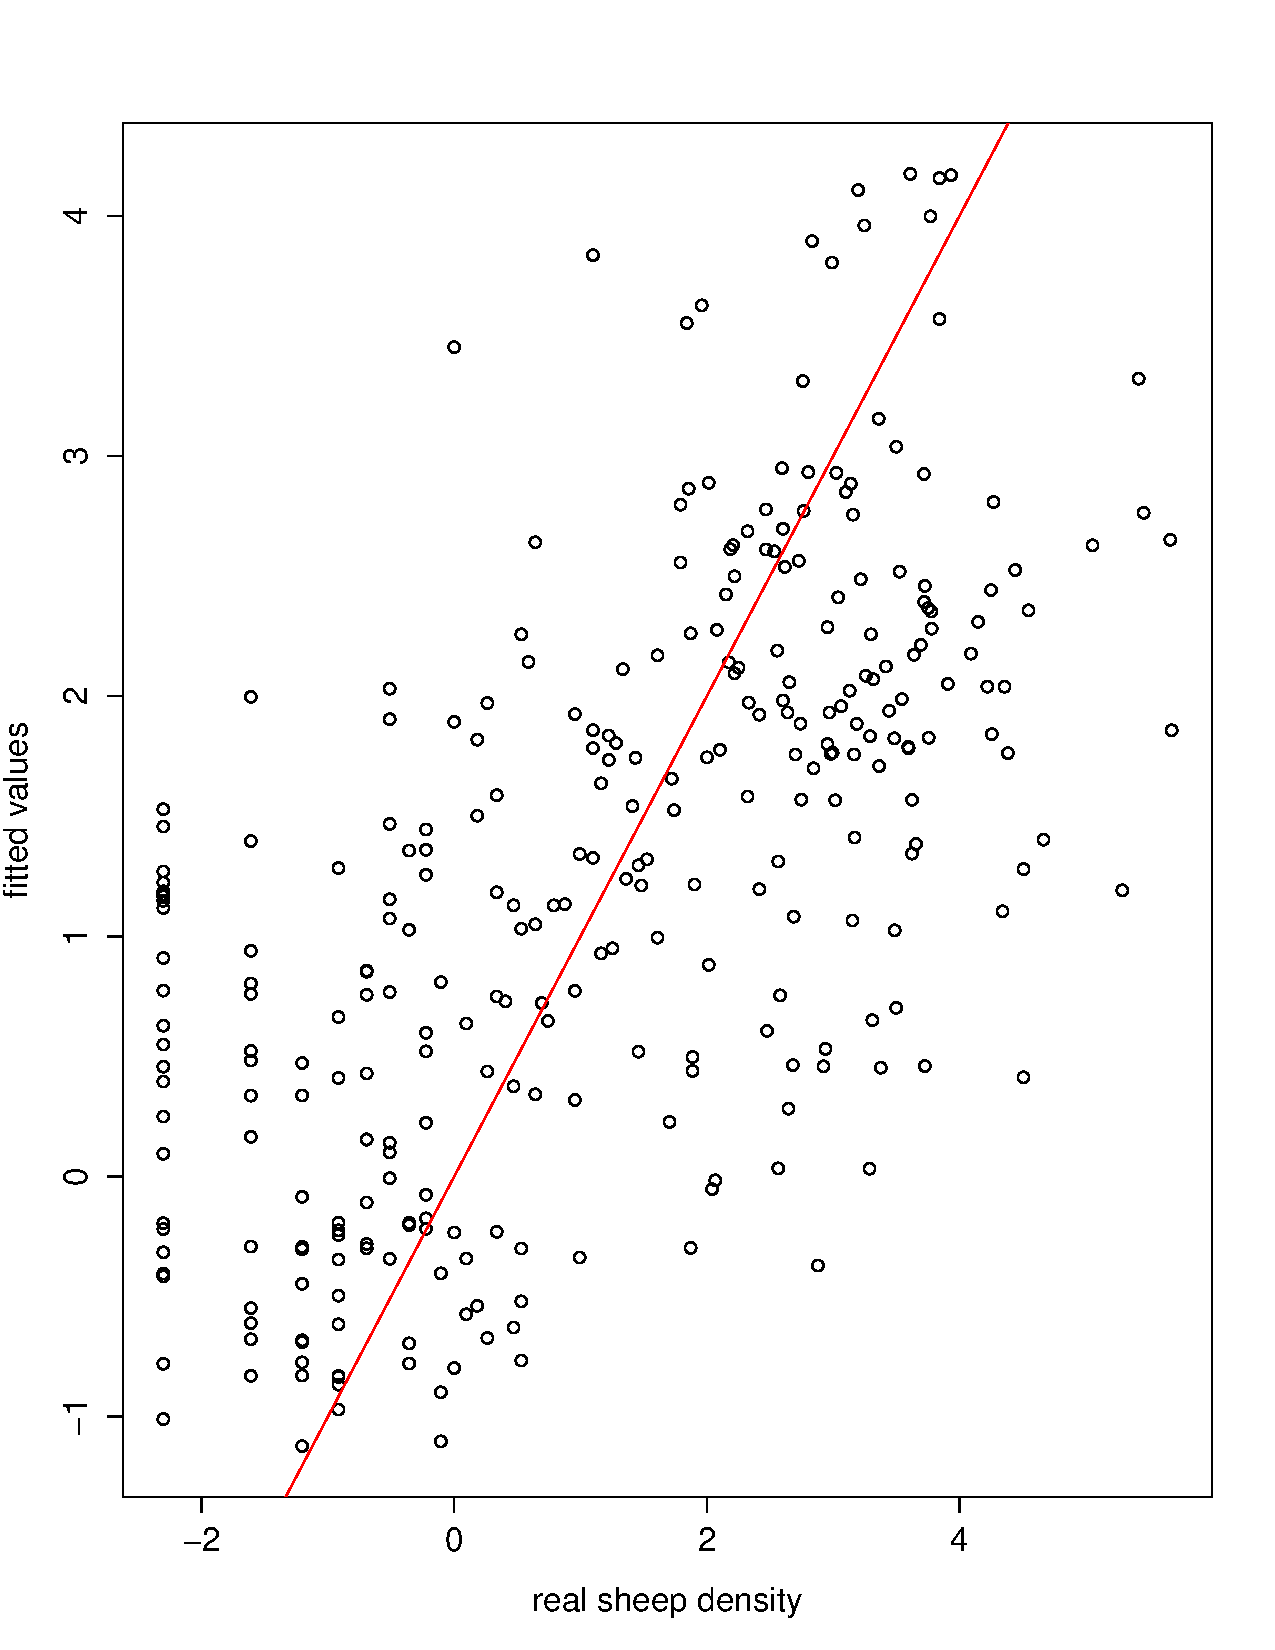
\includegraphics[width=\textwidth, height=6cm]{glm_ols_fit.pdf}
            \caption{fitted value plot with first 300 points}\label{glm_ols_fit}
        \end{subfigure}
        \caption{}
\end{figure}
\subsection{Attempt to Improve by TLS}

The model should be improved with the assumption that variance is increasing with $Y$.  I could use other GLM to fit the data. But there is a correlated problem.   Up to now, I analyzed each $y_i$ of $Y$ separately.  When analyzing one livestock density, influence caused by others is neglected in the above analysis.  For example, in the same area, if cattle density is high, then sheep density decreases and vice versa.  So it is better to analyze the whole livestock.  So I used total least square (TLS) regression.
\begin{equation*}
(Y + \Delta) = (X + \Xi)B
\end{equation*}
For TLS, we calculate $B$ which minimizes $\lambda||\Delta ||+ \kappa||\Xi||$.  Here I apply $Z = \log (Y + 1)$ to livestock to make data stationary and it makes the fitted values at least greater than -1 ($Y \geq e^Z -1$).  I set $\kappa = 10$ and $\lambda = 1$ because  X should not be modified too much. Therefore, more penalty is put on $\Xi$.  \reffig{tls_fit} shows the result.  The fitted values and true values are the sum of all livestock density.  The correlation is 0.6734.  So it improve 30\% compared with simple OLS.  \reffig{tls_res} shows our residuals are still dependent on livestock density, but the dependent relation is not as apparent as before.  The problem is how much weight should be put on each kind of livestock when summing.  Here I put equal weight, but actually resource to support one cattle may equivalently support two sheep or 5 hens.
\begin{figure}[h]
        \centering
        \begin{subfigure}[b]{0.475\textwidth}
            \centering
            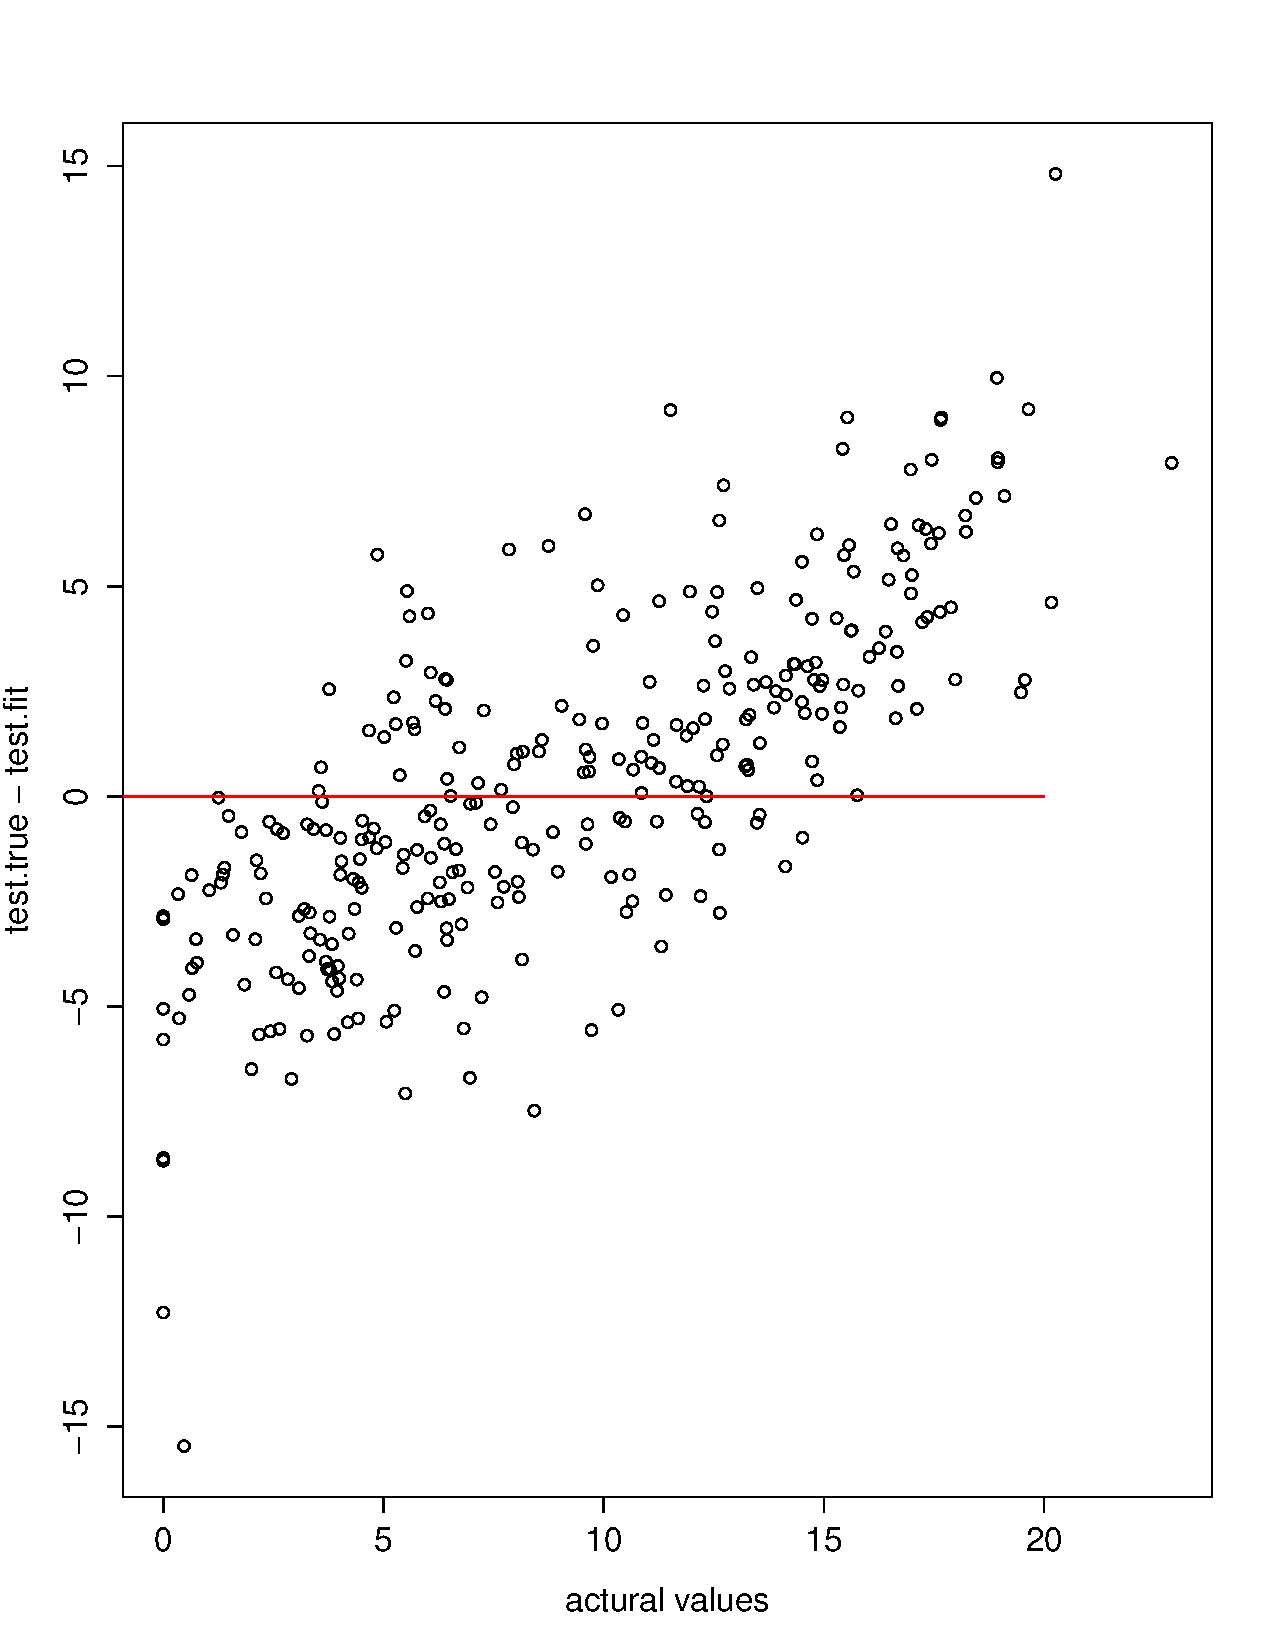
\includegraphics[width=\textwidth, height=6cm]{tls_res.pdf}
            \caption{residual plot with first 300 points}\label{tls_res}
        \end{subfigure}
        \quad
        \begin{subfigure}[b]{0.475\textwidth}
            \centering
            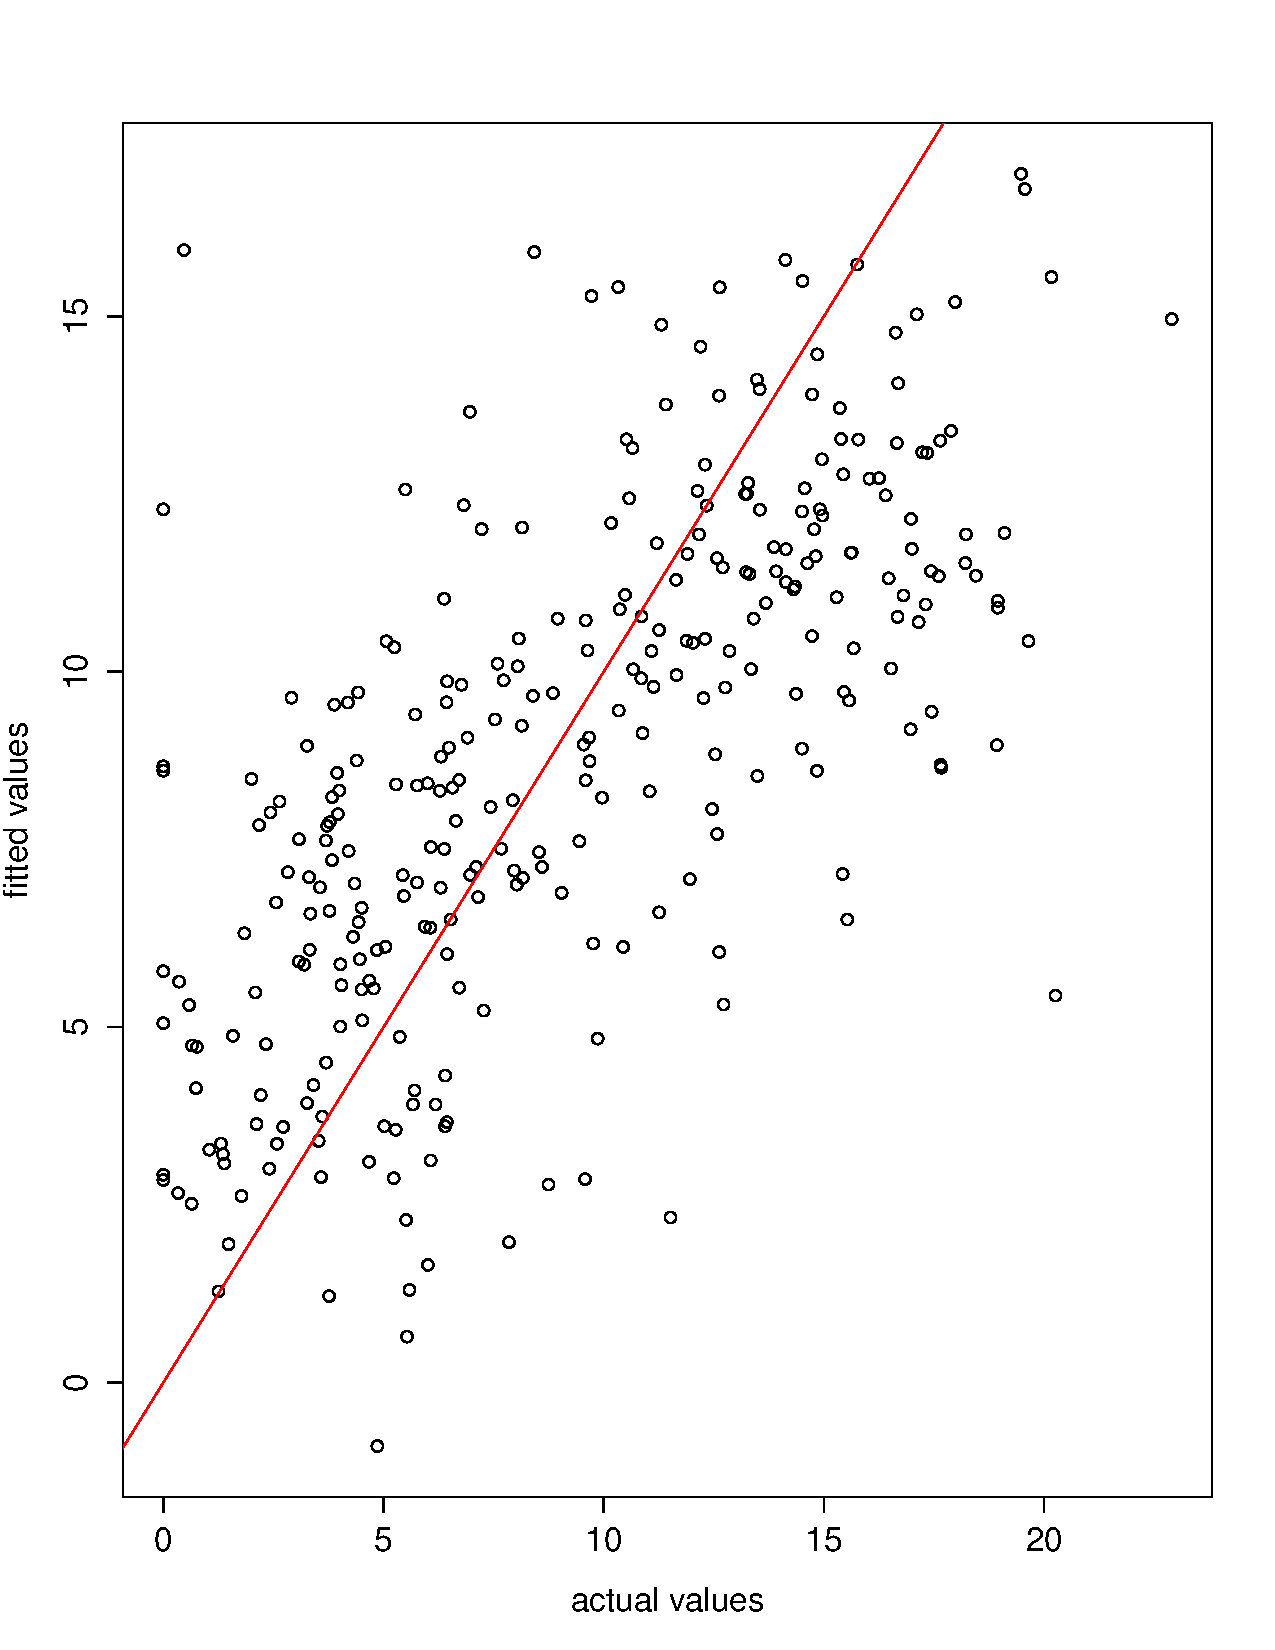
\includegraphics[width=\textwidth, height=6cm]{tls_fit.pdf}
            \caption{fitted value plot with first 300 points}\label{tls_fit}
        \end{subfigure}
        \caption{}
\end{figure}

\subsection{Apply Random Forest on Ecology System}
To classify ecology system with continuous data, logistic regression can be applied.  However, in the above section, I believed LR is not reliable.  So here I applied machining learning method, random forests.  Random Forest\cite{rand2} is a multitude of decision trees at training time and outputting the class that is the mode of the classes (classification) or mean prediction (regression) of the individual trees. Random decision forests correct for decision trees' habit of overfitting to their training set.\cite{rand1}
\begin{verbatim}
Call:
 randomForest(formula = ecol ~ ., data = temp, mtry = 6, 
                             ntree = 1000, na.action = na.omit)
               Type of random forest: regression
                     Number of trees: 1000
No. of variables tried at each split: 6

          Mean of squared residuals: 0.1256479
                    % Var explained: 97.23
\end{verbatim}
The result is shown that  97.23\% percent of variance is explained.  The accuracy of fitted values is 92.72\%.  So it is a better method than LR when the size of data is large and factors don't have linear relation.



\section{Social Facotrs}
Most social factors are discrete.  Regression cannot be applied.  So I mainly use correspondence analysis and analysis of variance. \par
\vspace{4mm}

There are 381 different markets and 26 ports.  I divided transportation into 8 levels and divided total production value per hectare (referred as pv/ha) into 11 levels.  First I studied the relation between production value and transportation time.  The following is the contingency table.
\begin{verbatim}
> table(transportation_time = TT_20K.factor,
                                   production_value_per_area=vp_ar.factor)
                   production_value_per_area
transportation_time    0    1    2    3    4    5    6    7    8    9   10
                  0  694 3679 6623 5611 3938 2886 1669  798  423  256  549
                  1  482 2033 2422 2428 2303 1444  818  373  147   71  148
                  2  213  767  630  712  717  424  301  134   51   37   56
                  3  121  336  210  212  256  147  102   55   14   13   12
                  4   88  138   66   73  140   71   37   21    2    2    4
                  5   25   42   23   24   50   21    8    2    0    1    1
                  6    5   12    8    8   33   11    3    0    1    0    0
                  7    1    7    3    5   16   14    5    2    1    0    0
\end{verbatim}
The p-value of $\chi$-square test is less than 2.2e-16, so the transportation time and production value are not independent.  In \reffig{cor_trans}, "Cn" represents the level of production value and "Rn"represents the level of transportation time.  "R1" are close to "C5" and "C6��.  It demonstrates that areas within 5-hour distance away from cities have food production value 1200 to 1500 \$ per hectare.  "R2-R11" are close to "C1-C3".  It demonstrates that areas,distance of which is more than 5-hour distance , have less production value 0 to 900  \$ per hectare.  \par
\vspace{4mm}
\begin{figure}[h]
        \centering
        \begin{subfigure}[b]{0.475\textwidth}
            \centering
            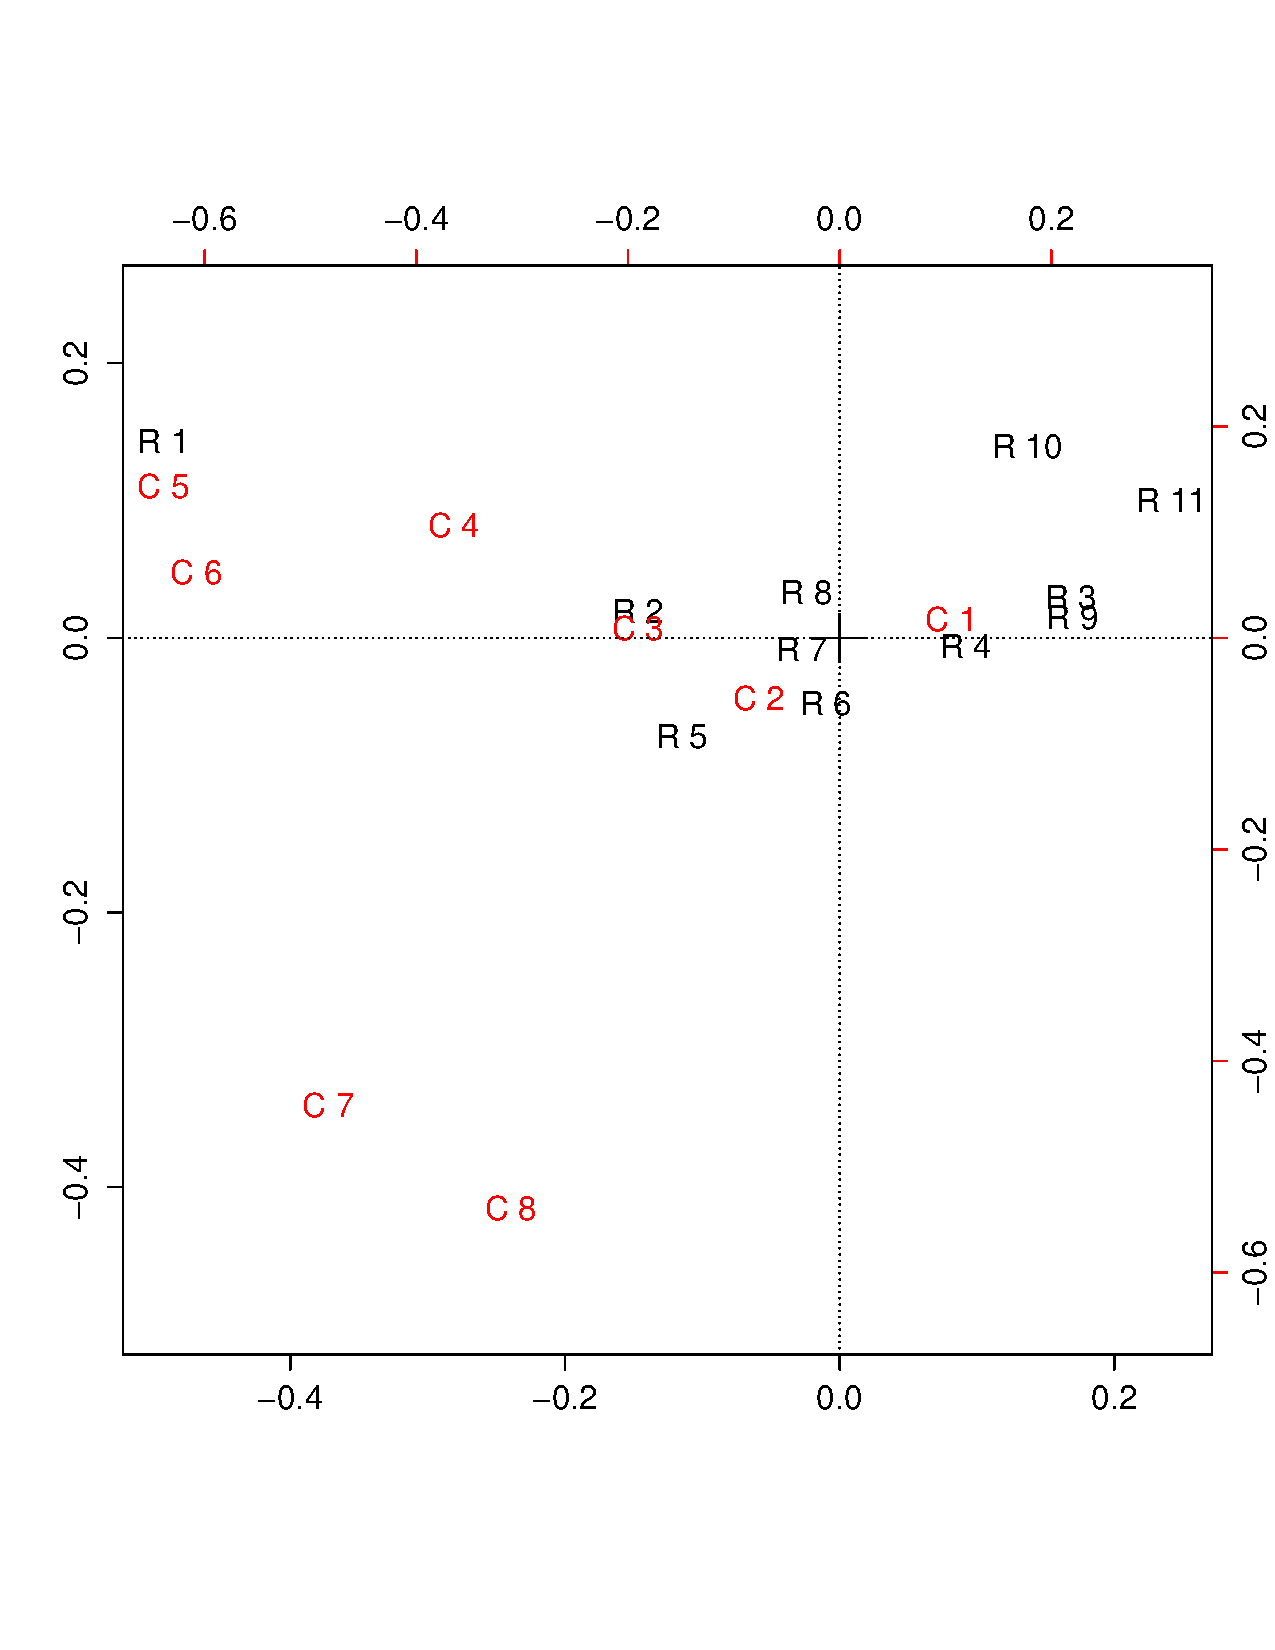
\includegraphics[width=\textwidth, height=6cm]{cor_trans.pdf}
            \caption{correspondence analysis for transportation time and production value}\label{cor_trans}
        \end{subfigure}
        \quad
        \begin{subfigure}[b]{0.475\textwidth}
            \centering
            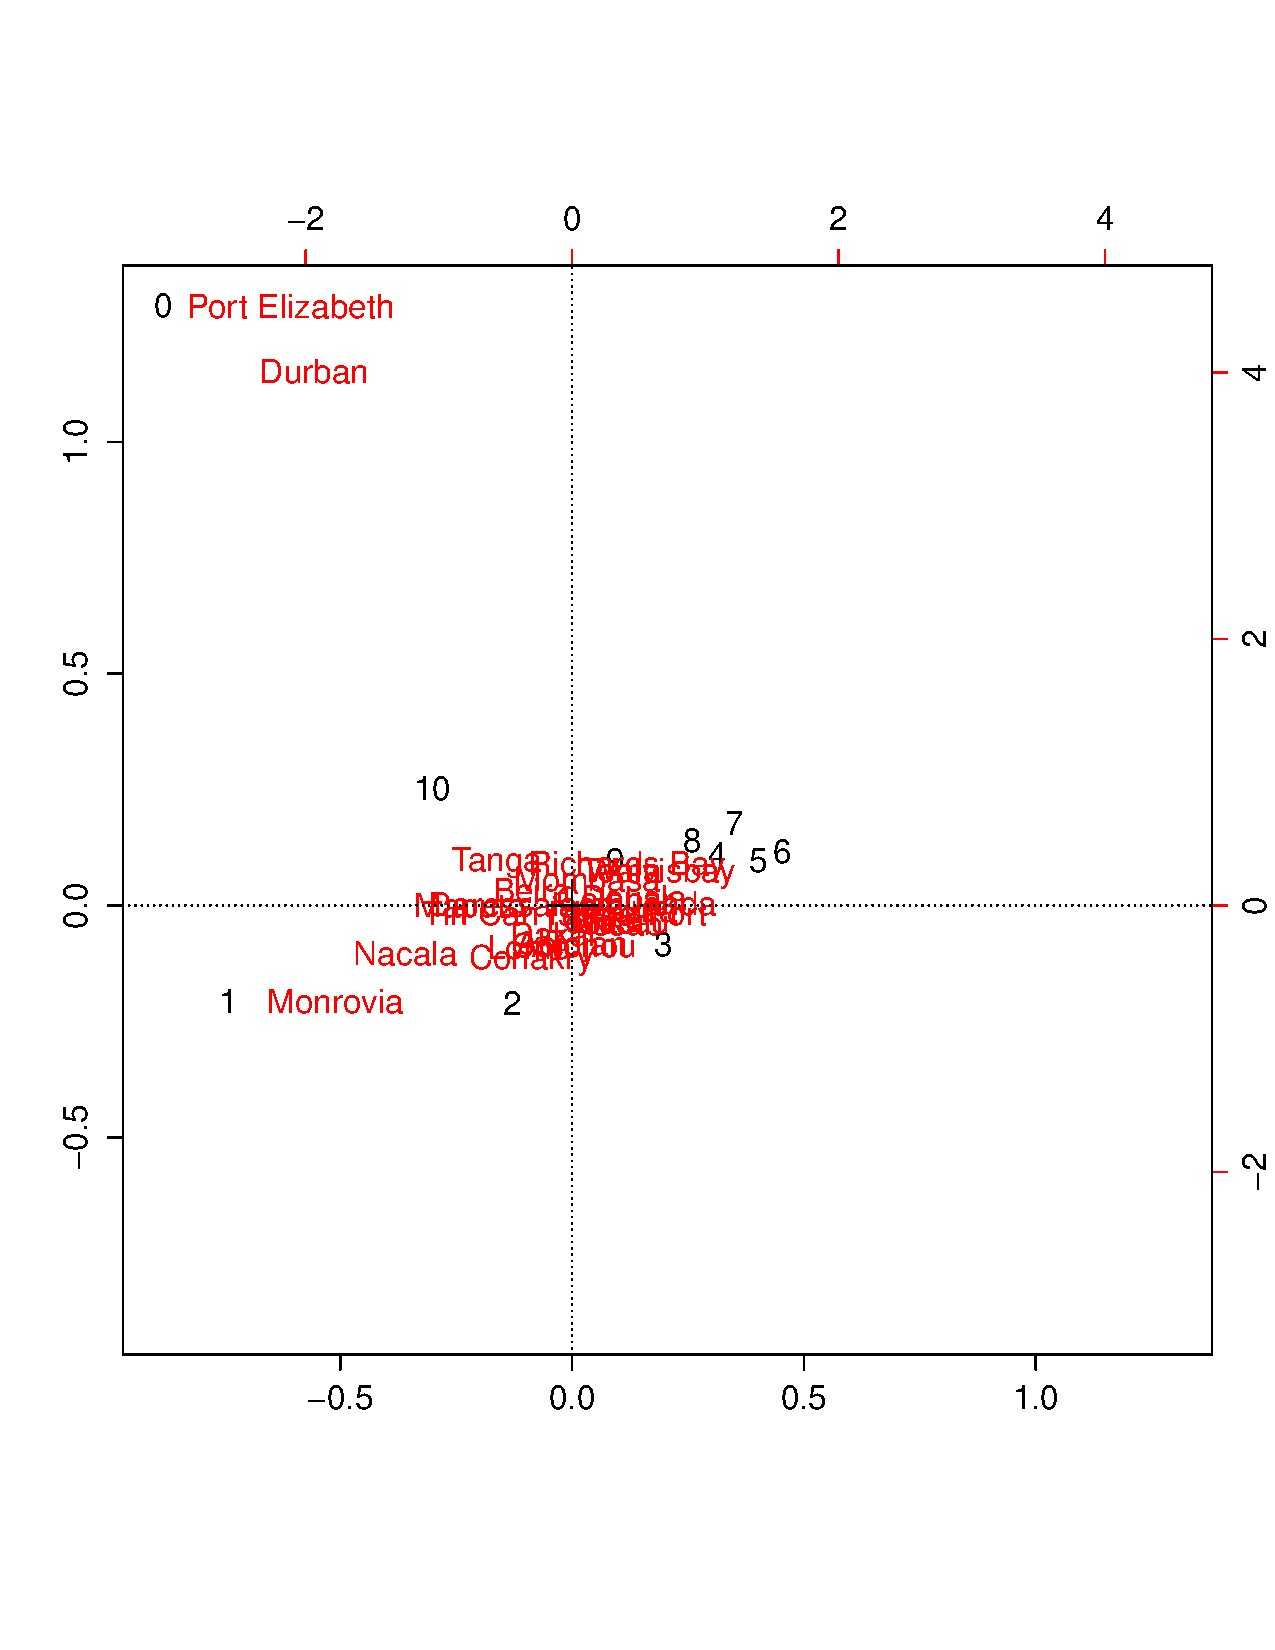
\includegraphics[width=\textwidth, height=6cm]{cor_port.pdf}
            \caption{correspondence analysis for ports and production value}\label{cor_port}
        \end{subfigure}
        \caption{}
\end{figure}
I used the similar method on relationship between ports and production value.  For this data, I deleted ports where all corresponding areas have 0 production value.  The p-value of $\chi$-square test is less than 2.2e-16, so ports and production value are not independent.  \reffig{cor_port} shows that the Elizabeth port and the Durban port don't give production value a bonus for corresponding areas.  Other ports at least guarantee most areas have production value grater than 300 \$ per hectare.  For relation between market and production value, I omit the similar result.  \par
\vspace{4mm}
It is not enough to have qualitative analysis.  I also researched how ports, markets and transportation time quantitatively influence the production value.  So I apply analysis of variance (ANOVA).
\begin{verbatim}
> summary(q)
               Df    Sum Sq  Mean Sq F value   Pr(>F)
market        380 7.275e+09 19144941  56.080  < 2e-16 ***
port           24 5.041e+07  2100249   6.152  < 2e-16 ***
tran.time       7 1.882e+07  2688415   7.875 1.43e-09 ***
Residuals   45877 1.566e+10   341385                     
\end{verbatim}
The mean square of residuals are too large.  And the interaction between those factors may also influence production value.  So a modified result with interaction of ports and transportation time is shown as follows:
\begin{verbatim}
> summary(q)
                  Df    Sum Sq  Mean Sq F value   Pr(>F)
market           380 7.275e+09 19144941  56.644  < 2e-16 ***
port              24 5.041e+07  2100249   6.214  < 2e-16 ***
tran.time          7 1.882e+07  2688415   7.954 1.11e-09 ***
port:tran.time   101 1.900e+08  1881601   5.567  < 2e-16 ***
Residuals      45776 1.547e+10   337986
\end{verbatim}
The mean square of residuals is not cut down significantly, so this modified method failed. \reffig{aov_res} and \reffig{aov_qq} shows small residuals follow normal distribution but high residuals don't.  Areas with high production value can have scale effect so that their production value can increase further.  So for further study, I need to establish at least 2 different distributions for the data and also research on how to classify data into different distributions.  Looking at degree of freedom, I added more interaction parts.  However, if interaction of transportation time and market is added, $7*380$ new factors will be introduced.  My laptop collapsed each time running the program.
\begin{figure}[h]
        \centering
        \begin{subfigure}[b]{0.475\textwidth}
            \centering
            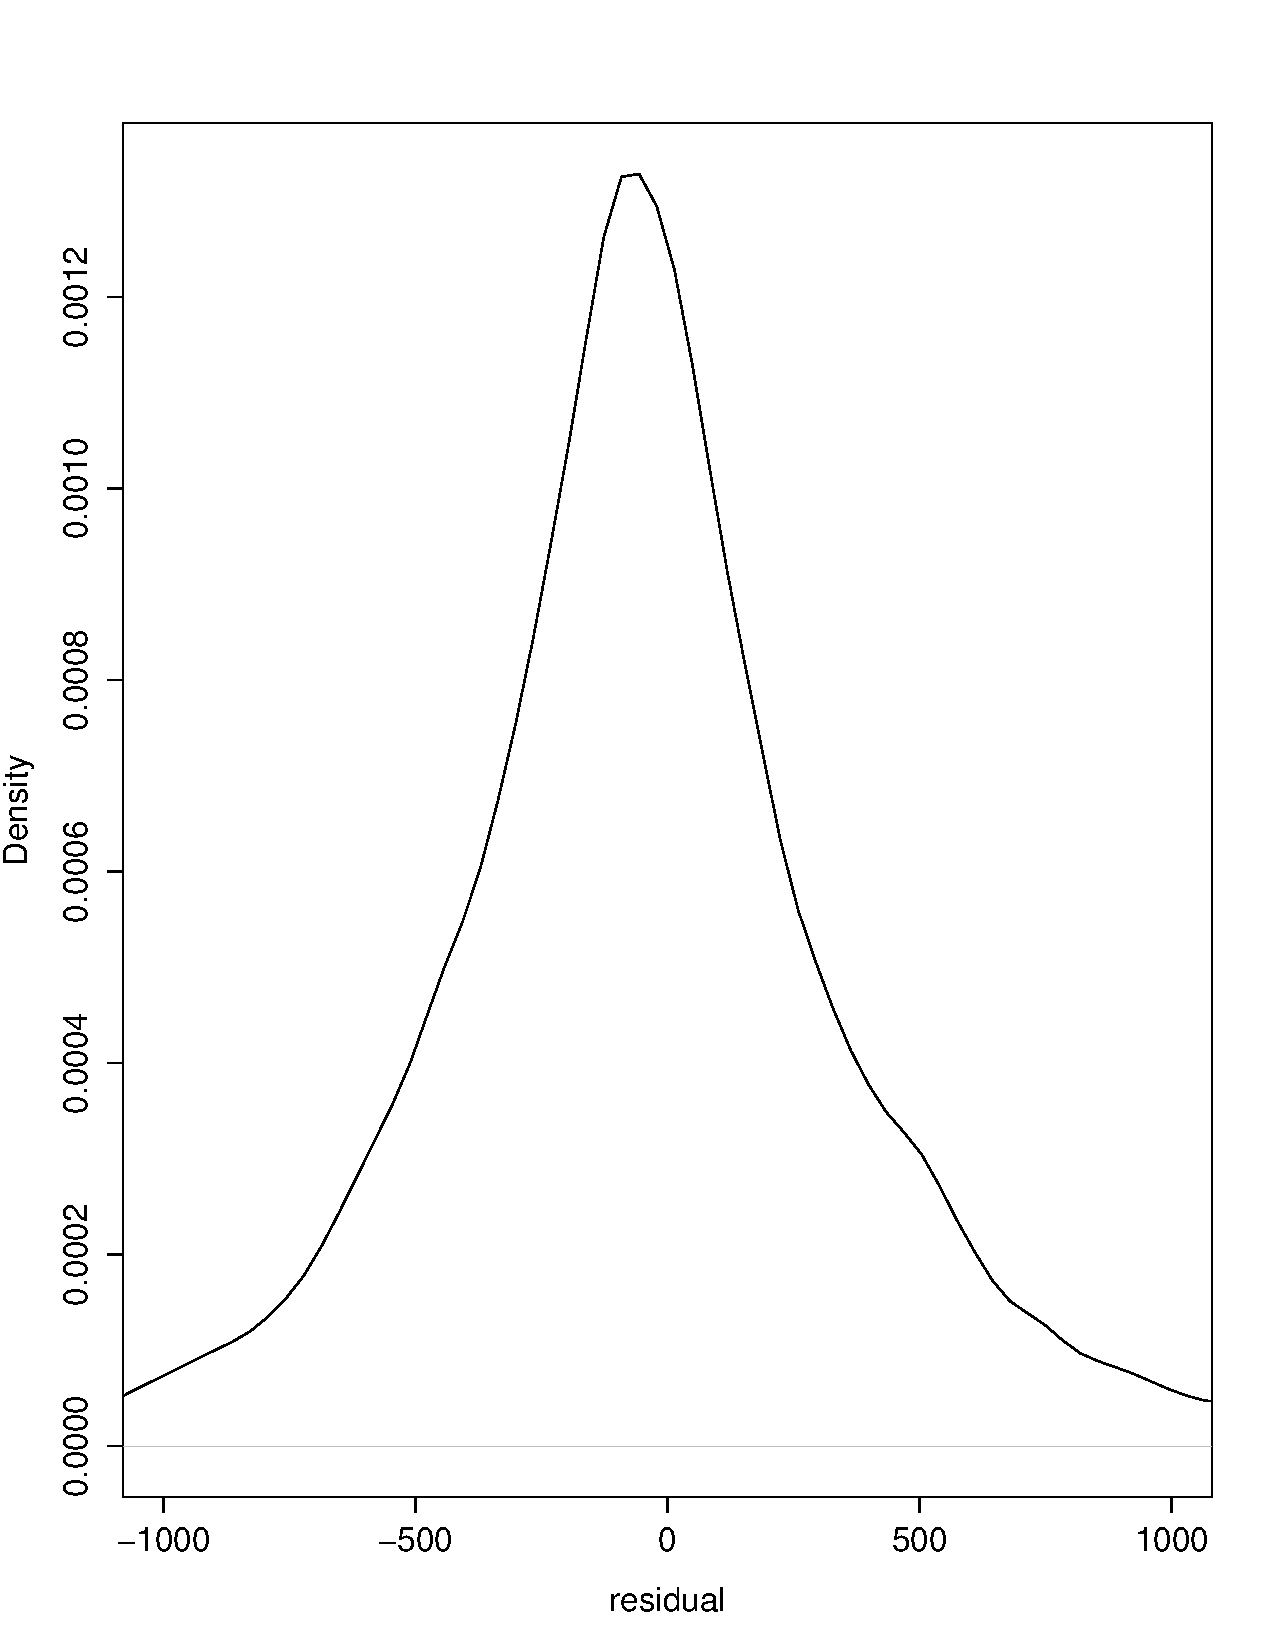
\includegraphics[width=\textwidth, height=6cm]{aov_res.pdf}
            \caption{density function of residuals}\label{aov_res}
        \end{subfigure}
        \quad
        \begin{subfigure}[b]{0.475\textwidth}
            \centering
            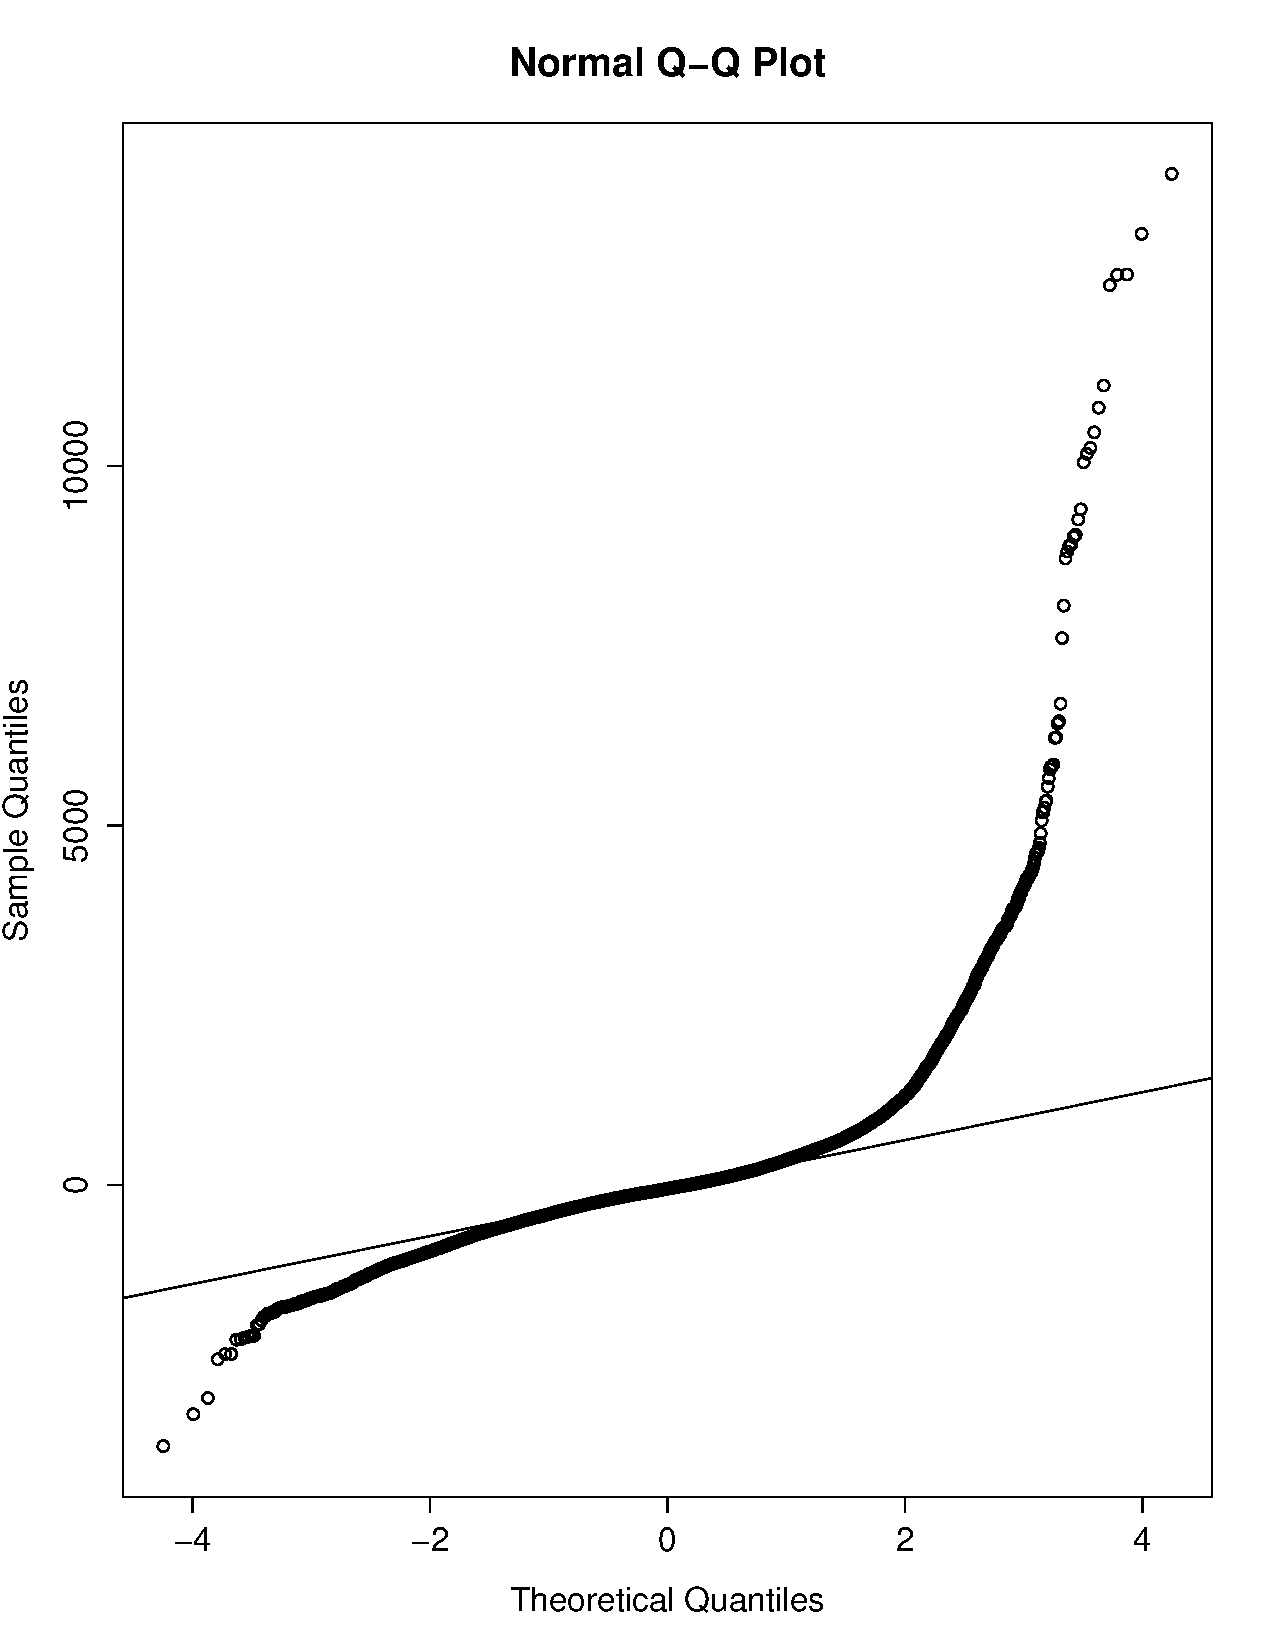
\includegraphics[width=\textwidth, height=6cm]{aov_qq.pdf}
            \caption{quantile-quantile plot}\label{aov_qq}
        \end{subfigure}
        \caption{}
\end{figure}



\section{Discussion}
\reffig{res_den} and \reffig{res_qq} show the density and quantile-quantile plots of residuals.  They are cheating.  It seems that our residual follows normal distribution.  However, when analyzing nature factors with livestock by total least square in section 2, we have seen that the variance is proportionate to total density.  So it is necessary to plot all graphs about residuals to check their independence and variance. \par
\vspace{4mm}
\begin{figure}[h]
        \centering
        \begin{subfigure}[b]{0.475\textwidth}
            \centering
            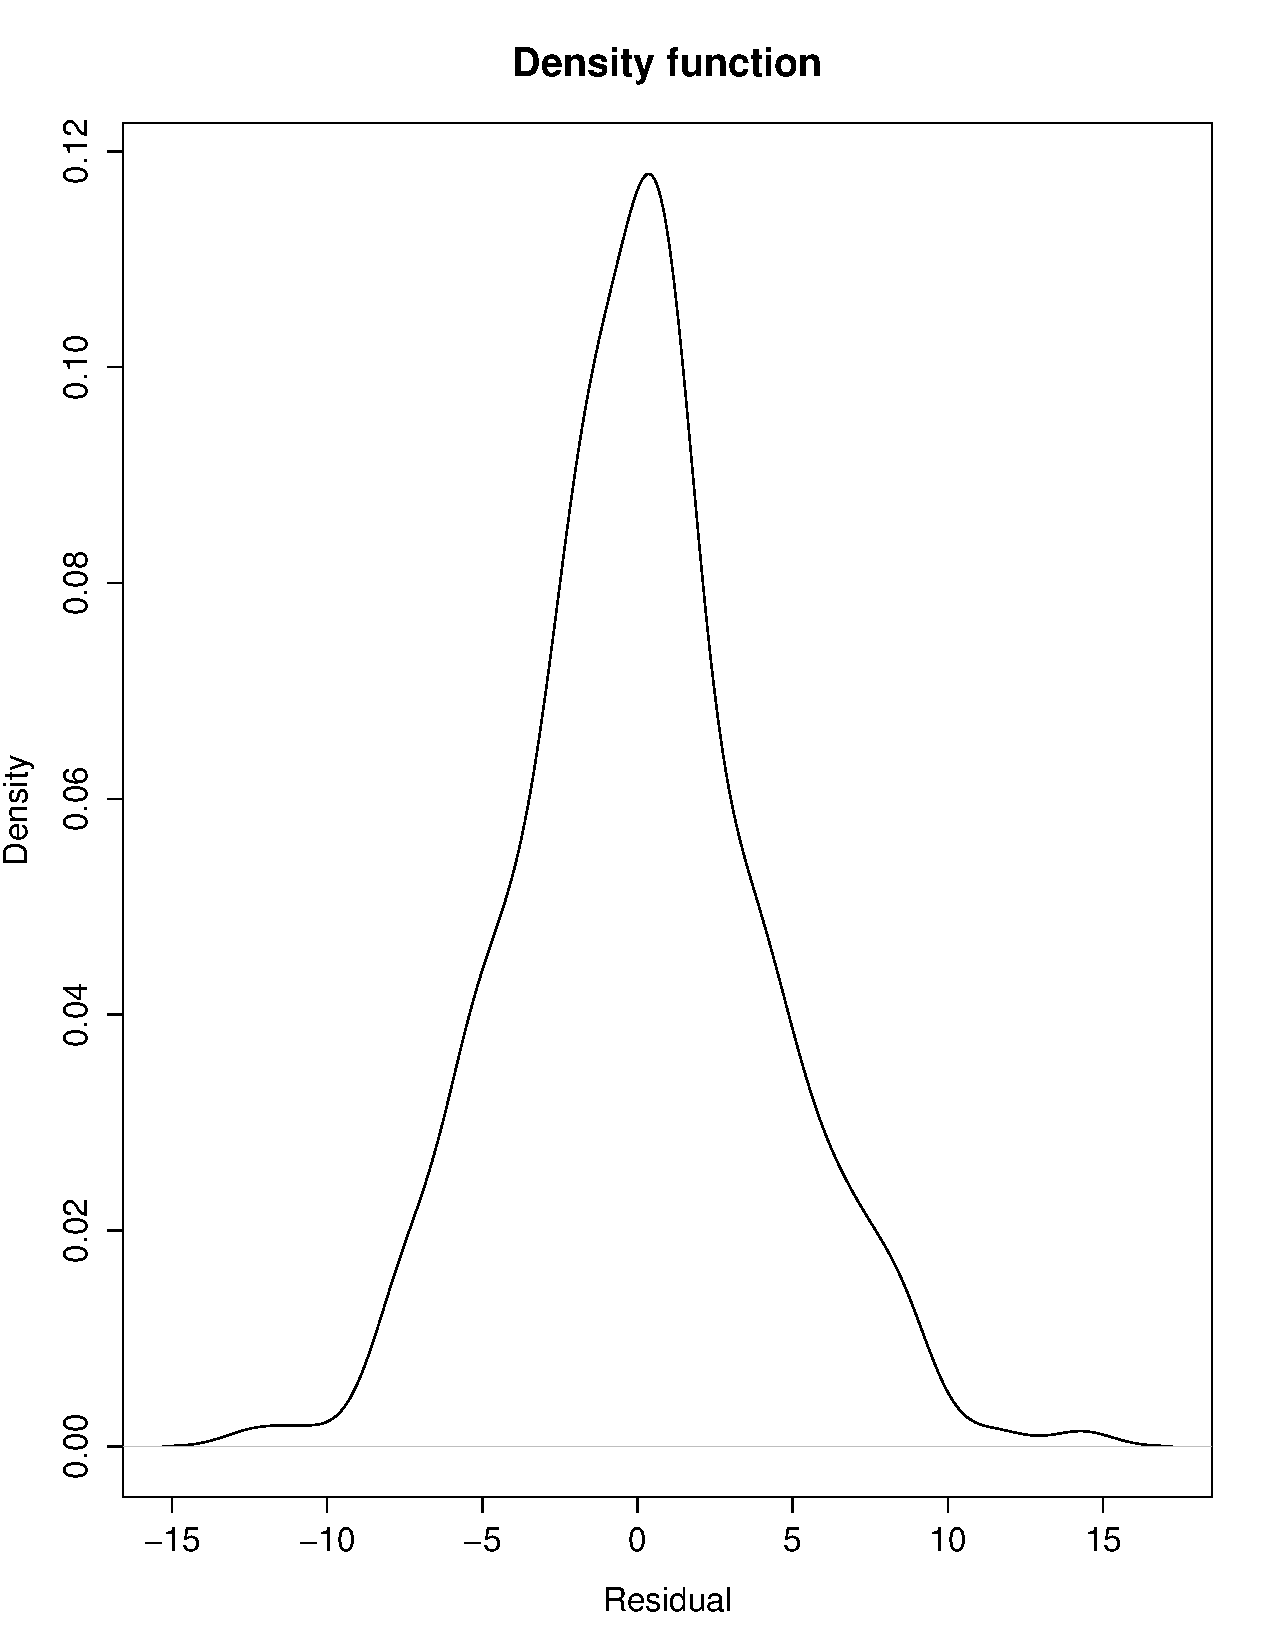
\includegraphics[width=\textwidth, height=6cm]{res_den.pdf}
            \caption{density function of residuals}\label{res_den}
        \end{subfigure}
        \quad
        \begin{subfigure}[b]{0.475\textwidth}
            \centering
            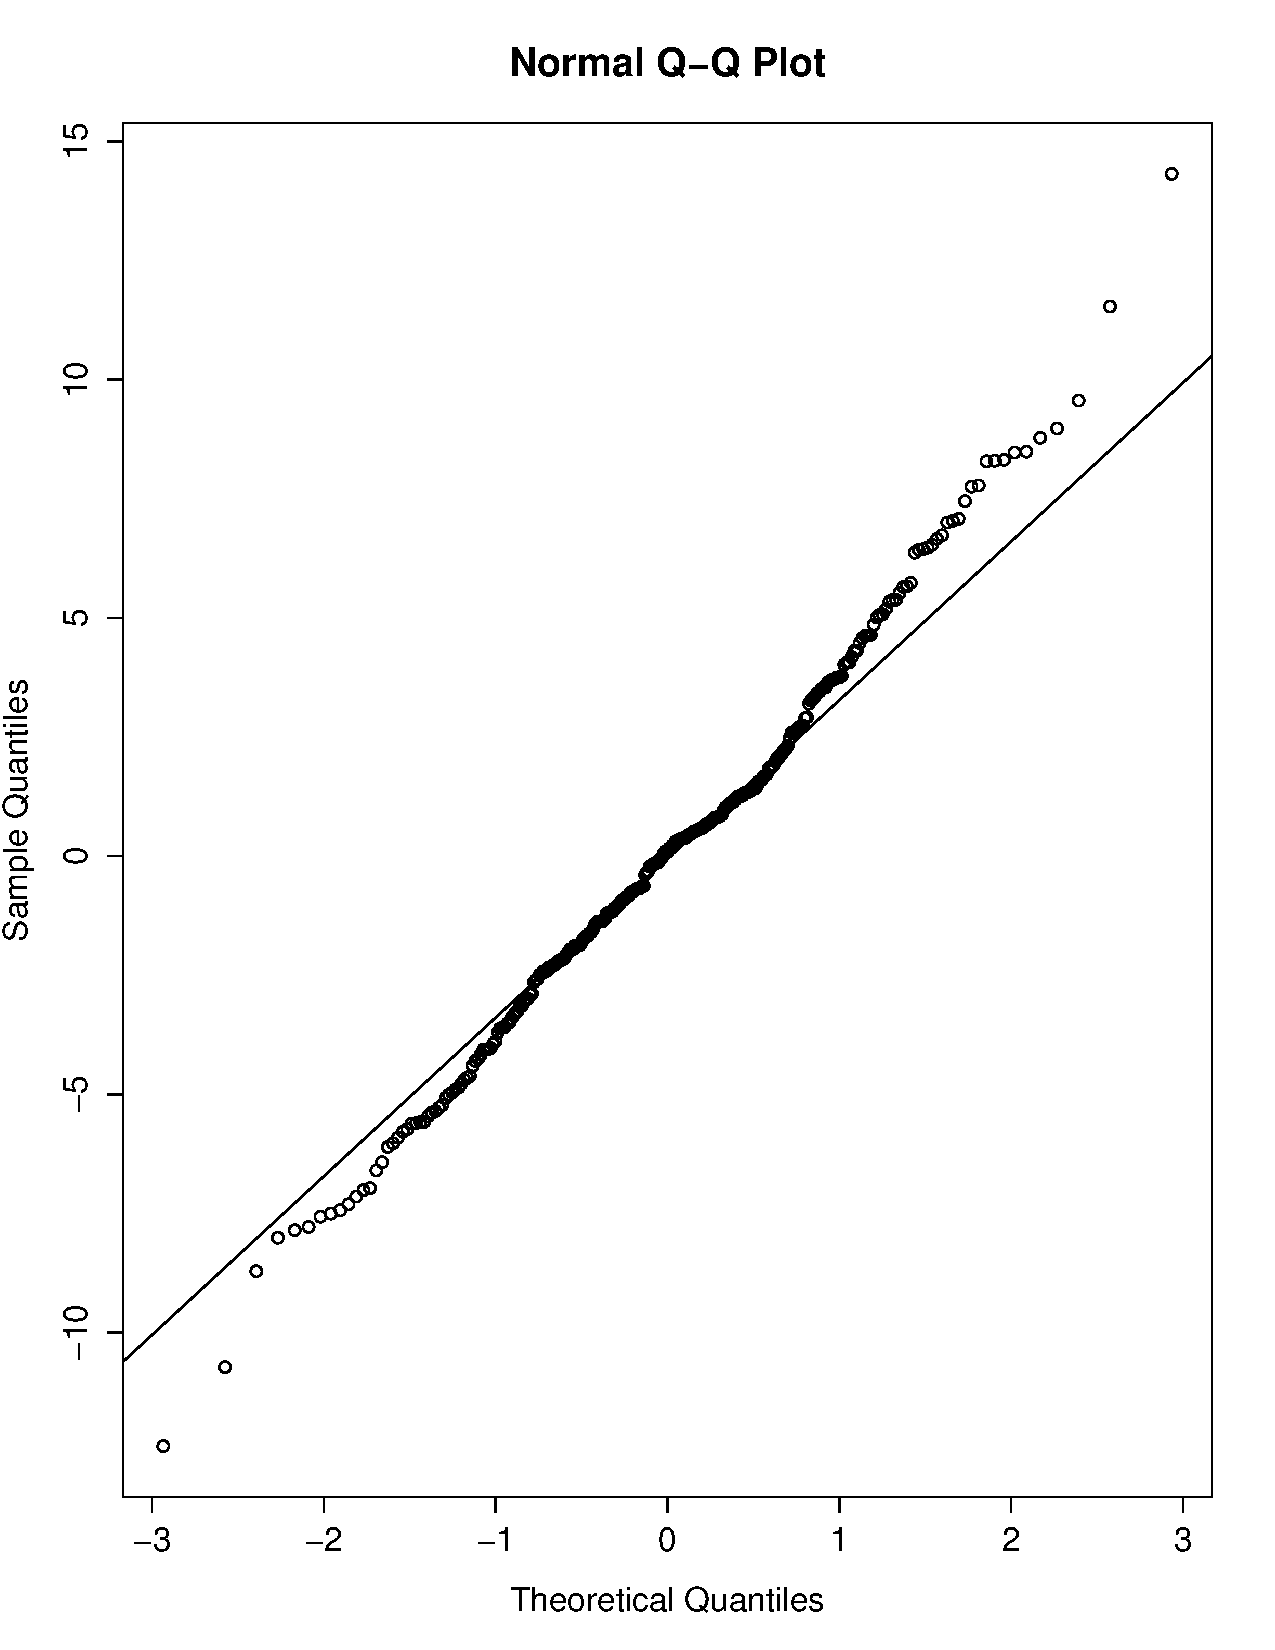
\includegraphics[width=\textwidth, height=6cm]{res_qq.pdf}
            \caption{quantile-quantile plot}\label{res_qq}
        \end{subfigure}
        \caption{}
\end{figure}

For the research, the number of original observations is 303453 while only 66322 are complete.  Most observations with missing data are from poor areas.  So the research is biased and may overestimate the natural and social effects on agriculture.  Besides, for poor areas, the data is hard to collect and collected data may not be as accurate as the one in rich areas.  In order to go over it, I suggest applying clustered sampling\cite{cluster sampling} for further survey.  In other words, choose several blocks of areas in Sahara randomly instead of dong a comprehensive survey in rich areas.  \par
\vspace{4mm}
I mainly applied regression, analysis of variance and matrix operation.  So most prediction is based on linear combination while those factors could have nonlinear relation with density.  Although I tried to add squared terms or interaction, the result is still frustrating (ANOVA shows this point).  So nonlinear model is recommended.  Based on the large data, I would like to try Kernel Method\cite{kernel ridge} if only prediction is needed.  This method is good at prediction based on nearby observation.  Also  generalized additive model\cite{gam} is another good choice if variables within natural and social factors are tested to be uncorrelated.  To achieve this, PCA can be applied.\par
\vspace{4mm}








\begin{thebibliography}{9}
\bibitem{World Population Prospects}
Department of Economic and Social Affairs Population Division, World Population Prospects The 2015 Revision, 2015
\bibitem{HarvestChoice}
HarvestChoice, International Food Policy Research Institute (IFPRI); University of Minnesota, 2016, "CELL5M: A Multidisciplinary Geospatial Database for Africa South of the Sahara", http://dx.doi.org/10.7910/DVN/G4TBLF, Harvard Dataverse, V2
\bibitem{kernel ridge}
Welling, M. (2013). Kernel ridge Regression. Max Welling��s Classnotes in Machine Learning (http://www. ics. uci. edu/welling/classnotes/classnotes. html), 1-3.
\bibitem{gam}
Hastie, T., \& Tibshirani, R. (1986). Generalized additive models. Statistical science, 297-310.
\bibitem{cluster sampling}
Thompson, S. K. (1990). Adaptive cluster sampling. Journal of the American Statistical Association, 85(412), 1050-1059. Chicago	
\bibitem{rand1}
Hastie, Trevor; Tibshirani, Robert; Friedman, Jerome (2008). The Elements of Statistical Learning (2nd ed.). Springer. ISBN 0-387-95284-5.
\bibitem{rand2}
Ho, Tin Kam (1995). Random Decision Forests (PDF). Proceedings of the 3rd International Conference on Document Analysis and Recognition, Montreal, QC, 14�C16 August 1995. pp. 278�C282.

\end{thebibliography}


\end{document}
